
Robotic workcell has to be designed keeping in mind the workspace of handling robot. Handling robot has to be able to reach every station in the workspace without any collision. 
The workcell is first developed in simulation with the use of \hyperref[acro:ROS]{ROS} and gazebo software. This reduced the development time as it allowed for quick changes to the workcell.

The preliminary designs for the robotic workcell were elaborated
in the form of \hyperref[acro:CAD]{CAD} models and successively converted into final \hyperref[acro:CAD]{CAD} designs. 
These \hyperref[acro:CAD]{CAD} models were later converted to suitable file format like \textit{.stl} and \textit{.dae} for the simulation software \hyperref[acro:ROS]{ROS}.
These meshes are then utilized to build up the whole workcell in \hyperref[acro:ROS]{ROS} and gazebo. Robot is defined in \hyperref[acro:URDF]{URDF} file format that includes
the physical description of the robot. \cite{urdf} This simulated environment in gazebo is used to update and fix the final layout of the robotic workcell.
Trajectories are planned to various subsystems in workcell using \hyperref[acro:ROS]{ROS} to determine to final position of robot in workcell.
Figure \ref{fig:robotic-workcell} shows the final layout of the workcell in gazebo software.
It consists of various subsystems which include bending machine, storage station, unloading station, handling robot, bending machine terminal operating robot and safety fence.

\begin{figure}[h]
    \centering
    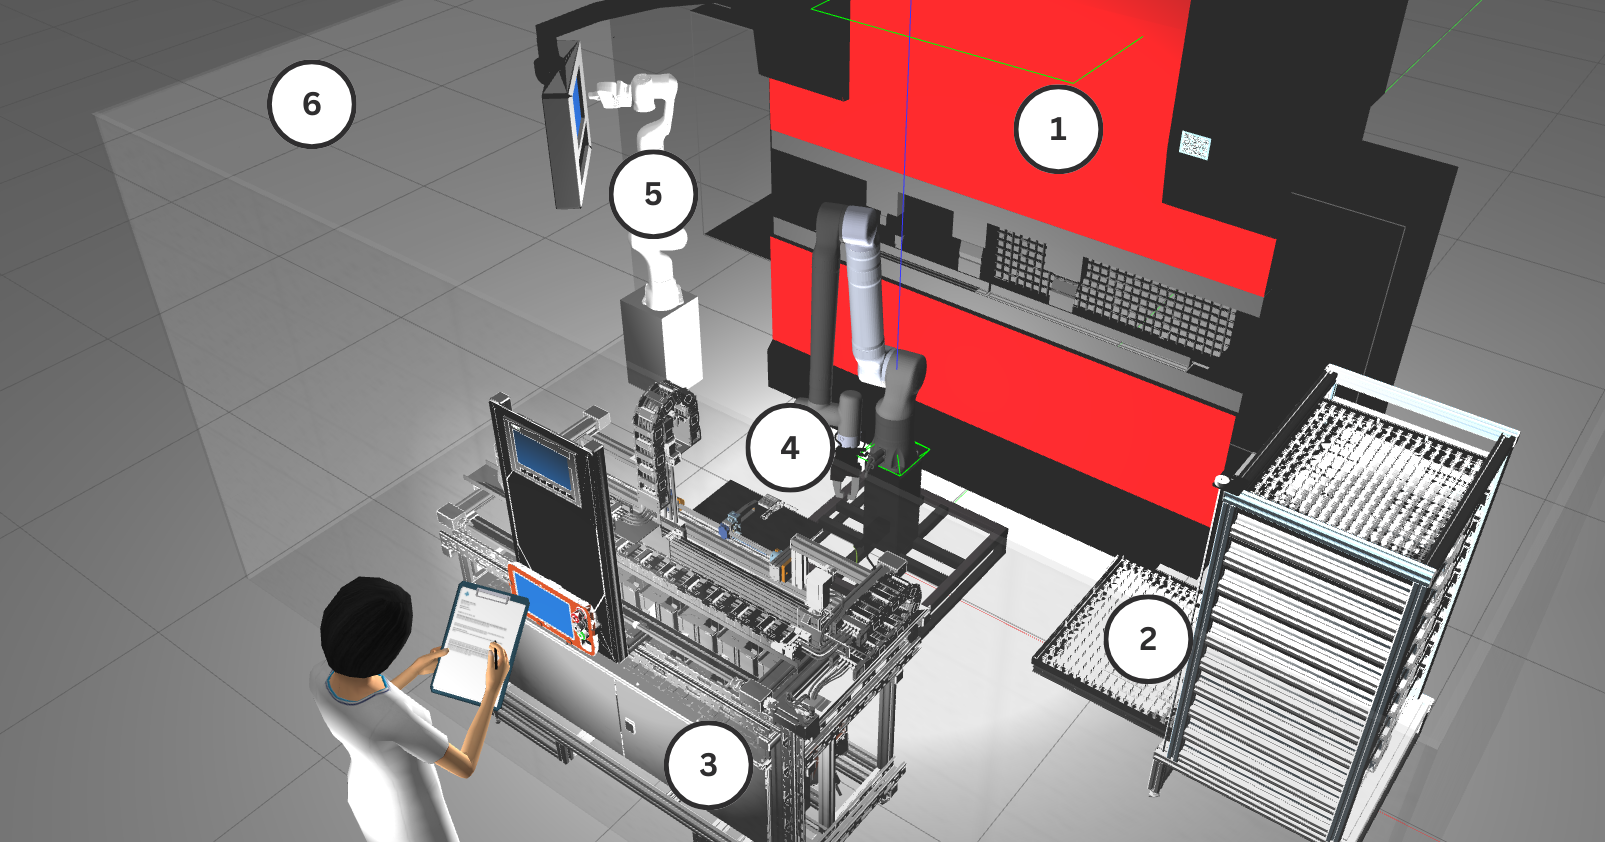
\includegraphics[width=\textwidth]{figures/robotic-workcell1.png}
    \caption{Robotic workcell layout. 1) Bending machine 2) Storage station 3) Unloading station 4) Handling robot 5) Bending machine terminal operating robot 6) Safety fence}
    \label{fig:robotic-workcell}
\end{figure}

The subsystems are described in more detail in the following
subsections. 


Sheets are loaded by workcell operator in the unloading station. Sheet metal parts are picked up by the handling robot and taken to bending machine to perform bending.
After all the bending operations are complete, sheet metal parts are stored in storage station.
The relation between each subsystem and the flow of energy, data, and material is shown in Figure \ref{fig:flow-workcell}.

% Create a figure of robotic workcell flow of things
\begin{figure}[h]
    \centering
    \begin{tikzpicture}[
        every node/.style={draw, ellipse, align=center, inner sep=5pt, line width=0.4mm},
        rect/.style={draw=cyan, rectangle, rounded corners=8pt, align=center, inner sep=12pt},
        energy/.style={->, >=stealth, thick, line width=0.5mm},
        data/.style={->, >=stealth, dashed, line width=0.5mm},
        material/.style={->, >=stealth, dotted, line width=0.5mm},
        node distance=1cm
    ]
      
        % Nodes
        \node (bending) [red] {\hyperref[sub:bending-machine]{Bending}\\ \hyperref[sub:bending-machine]{Machine}};
        \node (terminal) [red, left=of bending] {\hyperref[sub:bending-machine]{Terminal}};
        \node (camera1) [orange, below left=1cm and 0cm of bending] {\hyperref[sub:bending-machine]{Inspection}\\ \hyperref[sub:bending-machine]{Camera}};
        \node (footpedal) [red, below right=1cm and 0cm of bending] {\hyperref[sub:bending-machine]{Foot}\\ \hyperref[sub:bending-machine]{pedal}};
        \node (plc) [blue, below=4.5cm of bending, inner sep=10pt] {\hyperref[subsec:plc]{PLC}};
        \node (pandarobot) [gray, above left=0.5cm and 1.5cm of plc] {\hyperref[sub:panda-robot]{Panda}\\ \hyperref[sub:panda-robot]{Robot}};
        \node (handlingrobot) [green, above right=0.5cm and 3cm of plc] {\hyperref[sub:handling-robot]{Handling}\\ \hyperref[sub:panda-robot]{Robot}};
        \node (camera3) [green, above right=of handlingrobot] {\hyperref[sub:handling-robot]{Camera}};
        \node (storage) [rect, below=3cm of camera3, text=cyan] {\hyperref[sub:storage-station]{Storage}\\ \hyperref[sub:storage-station]{Station}};
        \node (camera2) [gray, above left=of pandarobot] {\hyperref[sub:panda-robot]{Camera}};
        \node (unloading) [rect, below=of plc, draw=cyan, text=cyan] {\hyperref[sub:unloading-station]{Unloading}\\ \hyperref[sub:unloading-station]{Station}};
        \node (energy) [rectangle, draw=none, fill=white, text width=2.5cm, align=left, above left=0.3cm and 0cm of unloading, font=\footnotesize] {Energy Flow};
        \node (data) [rectangle, draw=none, fill=white, text width=2.5cm, align=left, below=0cm of energy, font=\footnotesize] {Data Flow};
        \node (material) [rectangle, draw=none, fill=white, text width=2.5cm, align=left, below=0cm of data, font=\footnotesize] {Material Flow};
        \node (energy_left) [circle, draw=none, left=0cm of energy] {};
        \node (energy_right) [circle, draw=none, left=1cm of energy_left] {};
        \node (data_left) [circle, draw=none, left=0cm of data] {};
        \node (data_right) [circle, draw=none, left=1cm of data_left] {};
        \node (material_left) [circle, draw=none, left=0cm of material] {};
        \node (material_right) [circle, draw=none, left=1cm of material_left] {};
        
        % Energy flow
        \draw[energy] (bending) -- (terminal);
        \draw[energy] (bending) -- (footpedal);
        \draw[energy, transform canvas={xshift=-4pt}] (plc) -- (camera1);
        \draw[energy] (plc) .. controls ++(-1, 0) and ++(1,-1) .. (pandarobot);
        \draw[energy] (pandarobot) .. controls ++(-1, 0.5) and ++(0.5,-1) .. (camera2);
        \draw[energy] (plc) .. controls ++(1, 0) and ++(-1,-1) .. (handlingrobot);
        \draw[energy] (handlingrobot) .. controls ++(2,1.2) and ++(-2,-1.3) .. (camera3);
        \draw[energy, transform canvas={xshift=-4pt}] (unloading) -- (plc);
        
        % Data flow
        \draw[data] (terminal) .. controls ++(-2,-1) and ++(0,1) .. (camera2);
        \draw[data] (camera2) .. controls ++(1, -0.5) and ++(-1,1) .. (pandarobot);
        \draw[data] (camera3) .. controls ++(-0.5,-1) and ++(2,0.5) .. (handlingrobot);
        \draw[data] (bending) -- (camera1);
        \draw[data] (plc) -- (footpedal);
        \draw[data] (storage) -- (camera3);
        \draw[data] (bending) .. controls ++(5,1) and ++(0,2) .. (camera3);
        \draw[data, transform canvas={xshift=4pt}] (camera1) -- (plc);
        \draw[data, <->, transform canvas={xshift=4pt}] (unloading) -- (plc);
        \draw[data, <->] (plc) .. controls ++(-1, 0.5) and ++(2,-1) .. (pandarobot);
        \draw[data, <->] (plc) .. controls ++(1, 0.4) and ++(-2,-1) .. (handlingrobot);
        \draw[data] (unloading) .. controls ++(8,0) and ++(4,-7) .. (camera3);
        \draw[data] (footpedal) .. controls ++(-0.5,1) and ++(1,-1) .. (bending);

        % Material flow
        \draw[material] (unloading) .. controls ++(2,1) and ++(1,-3) .. (handlingrobot);
        \draw[material] (handlingrobot) .. controls ++(1.5,-0.5) and ++(-1,1) .. (storage);
        \draw[material, <->] (bending) .. controls ++(4,-1) and ++(0,3) .. (handlingrobot);

        % Create legend for the figure
        \draw[energy,-] (energy_left) -- (energy_right);
        \draw[data,-] (data_left) -- (data_right);
        \draw[material,-] (material_left) -- (material_right);

    \end{tikzpicture}
    \caption{Energy, data and material flow in the robotic workcell}
    \label{fig:flow-workcell}
\end{figure}



\subsection{Bending machine}
\label{sub:bending-machine}

Bending machine as a unit comes with a terminal and a foot pedal. Terminal is used to operate
the bending machine for starting, stopping and configuring the bending machine and also loading the bending program.
Foot pedal comes with two pedals, one for closing the bending machine and other for opening of the bending machine.
Opening and closing of bending machine is controlled by a foot pedal for the manual bending operations.

\begin{figure}[h]
    \centering
    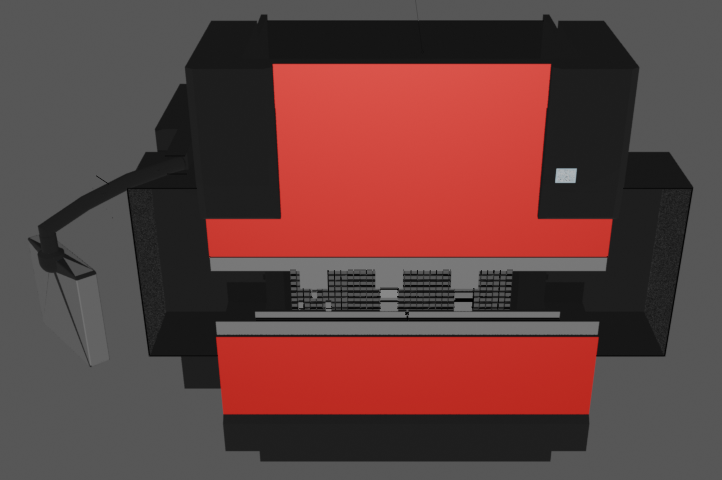
\includegraphics[width=0.75\textwidth]{figures/bending-machine-blender.png}
    \caption{Bending machine asset in simulation}
    \label{fig:bending-machine-blender}
\end{figure}
To automate the bending machine, \hyperref[acro:PLC]{PLC} is used to send signals to foot pedal which in turn, controls the opening and closing of bending machine.

An inspection camera is also added to measure the bending angle after each bending operation. This inspection camera is operated by the \hyperref[acro:PLC]{PLC}
and the bending angles are saved in \textit{.csv} file format and displayed on an \hyperref[acro:HMI]{HMI}.


\subsection{Storage station}
\label{sub:storage-station}
The storage station is a shelf with 10 drawers. The drawers of the shelf can be automatically opened and closed by the
handling robot. It is a mechanical system which is used to store final bended sheet metal parts.

\begin{figure}[h]
    \centering
    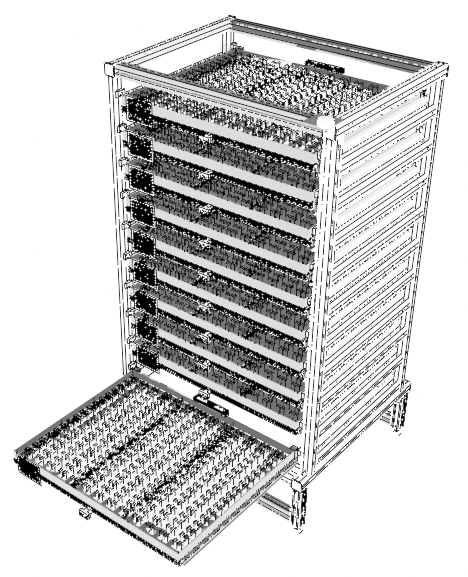
\includegraphics[width=0.3\textwidth]{figures/storage-station-blender.png}
    \caption{Storage Station asset in simulation}
    \label{fig:storage-station}
\end{figure}

When the storage station is full, human operators are to replace a filled shelf with a new empty shelf with a forklift. Thus, this is the only station
which is not fixed in the robotic workcell. The robotic camera mounted on the handling robot needs to determine the correct position of the storage station
after each restart.

\subsection{Unloading station}
\label{sub:unloading-station}
The task of the removal station is to take a single sheet metal part from a stack of raw sheets and make it
available to the robot unit. This is a mechatronic system with several different components, which all
have to function individually, but also together in combination. The mechatronic system is controlled by the PLC.


\begin{figure}[h]
    \centering
    \begin{subfigure}{0.505\textwidth}
        \centering
        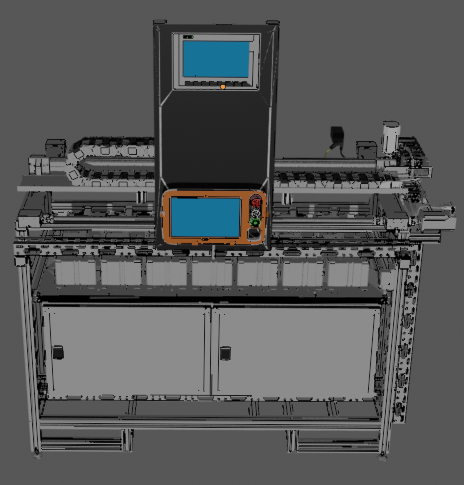
\includegraphics[width=\textwidth]{figures/unloading-station-front-blender.png} % Replace with your image file
        \caption{front-view}
        \label{fig:unloading-station-front}
    \end{subfigure}\hfill
    \begin{subfigure}{0.45\textwidth}
        \centering
        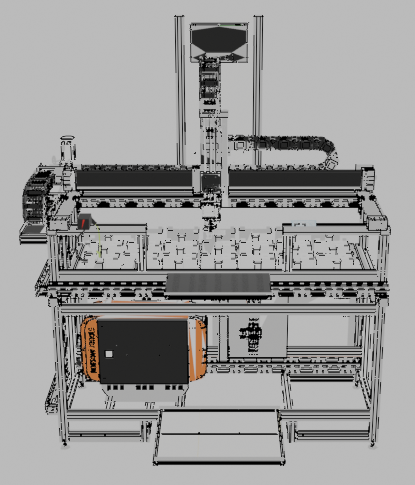
\includegraphics[width=\textwidth]{figures/unloading-station-back-blender.png} % Replace with your image file
        \caption{back-view}
        \label{fig:unloading-station-back}
    \end{subfigure}
    \caption{Unloading station in simulation}
    \label{fig:unloading-station}
\end{figure}

This unloading station is on top of a cabinet which houses the PLC and controller of the handling robot.


\subsection{Handling robot}
\label{sub:handling-robot}
\begin{figure}[h]
    \centering
    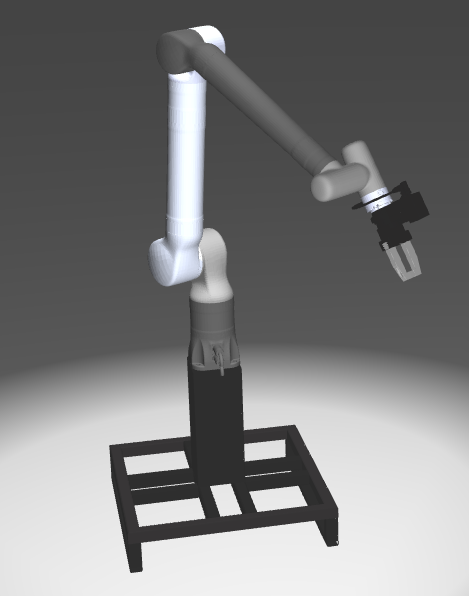
\includegraphics[width=0.3\textwidth]{figures/handling-robot-simulation.png}
    \caption{Handling Robot KR1410 in simulation}
    \label{fig:handling-robot-simulation}
\end{figure}
Handling robot is the primary robot which handles the sheet metal parts to different subsystems \textit{i.e.}
unloading station, bending machine and storage station.
It coordinates with the \hyperref[acro:PLC]{PLC} to make decisions during the execution of the program. Reachability
is very important in this case, as it should be able to handle sheet metal parts in any orientation.
A two finger gripper is used for grasping the sheet metal parts.

To get accuracy with the bending process, detection of features on the sheet metal parts is required.
A robotic camera is mounted of the robot for this purpose. In this way, handling robot can be trained 
to operate with different variants of sheet metal parts.

\hyperref[acro:ROS]{ROS} simulations of the handling robot is done to determine the performance of robot in the workcell.
The drawers of storage system is especially close
to the production floor and the robot requires some space to move around without getting stuck. 
Reachability is tested with the simulation of trajectories before the final integration of the real robot
in the workcell.

\subsection{Bending machine terminal operating robot}
\label{sub:panda-robot}
Together with the company \textbf{VisCheck GmbH}, an operating unit is developed
for entering parameters on the operating terminal and reading relevant values on the operating
terminal of the bending machine. The unit consists of a franka emika robot, a camera for reading terminal values
and a computer for controlling the robot. A touch screen pointer is attached to the gripper of the robot
for operating the touch screen of terminal.

\begin{figure}[h]
    \centering
    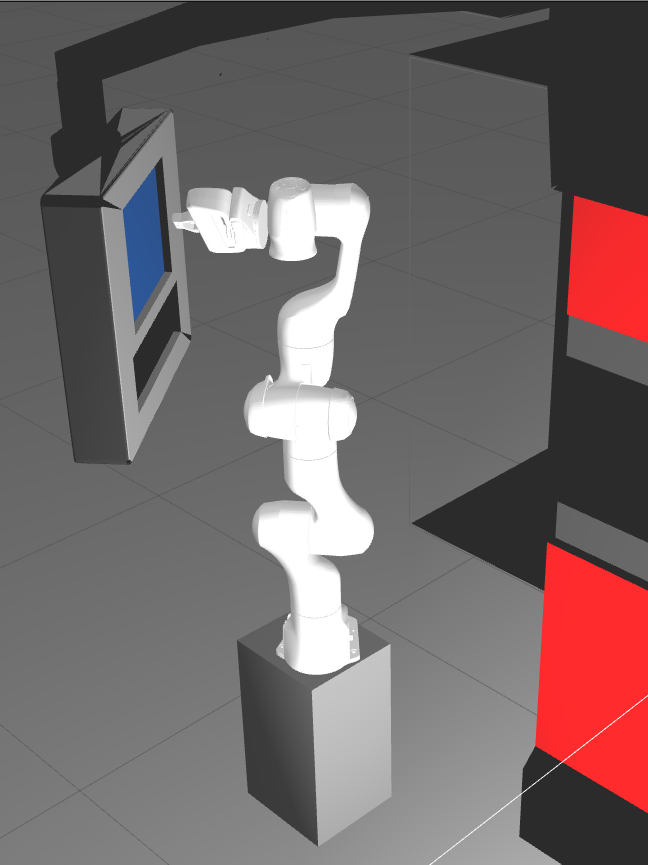
\includegraphics[width=0.3\textwidth]{figures/panda-robot-simulation.png}
    \caption{Franka emika panda robot as terminal operating robot in simulation}
    \label{fig:terminal-robot}
\end{figure}

As it is programmed by another company, it is not simulated in the software and not coordinated for any trajectory planning. Sufficient floor space
is left near the terminal of bending machine in the robotic workcell for the installation of this robot.
The trajectories of handling robot are not planned anywhere near this robot. To set this up, safety zone is created
during the programming of the handling robot.


\subsection{Safety fence}
\label{sub:safety-fence}
Safety fence marks the boundary of the robotic workcell. Even though the robot finalized is a collaborative robot,
bending machine poses a safety concern as it is operated automatically by the \hyperref[acro:PLC]{PLC}. The sheet metal parts are sharp
around the corners and when handled by the robot is deemed as not safe.

Two doors are installed for an entry in the robotic workcell. One is close to the storage system and is used
to move shelf in-and-out of the workcell by a forklift. The doors are installed with a safety mechanism such that if the door is open, the whole robot unit and bending machine cannot operate. This safety mechanism 
is again controlled by the \hyperref[acro:PLC]{PLC}. Safety fence is only installed at the end of the project by the company.
A simulation of the fence with \hyperref[acro:ROS]{ROS} and gazebo is not necessary in this case and is not included as assets in gazebo.

